\section{Информация}

149 ФЗ об информации, информационных законах и защите информации

\textbf{Информация} -- сведения, независимые от формы представления.

\subsection{Стадия жизни информаиции}

\begin{figure}[H]
    \centering
    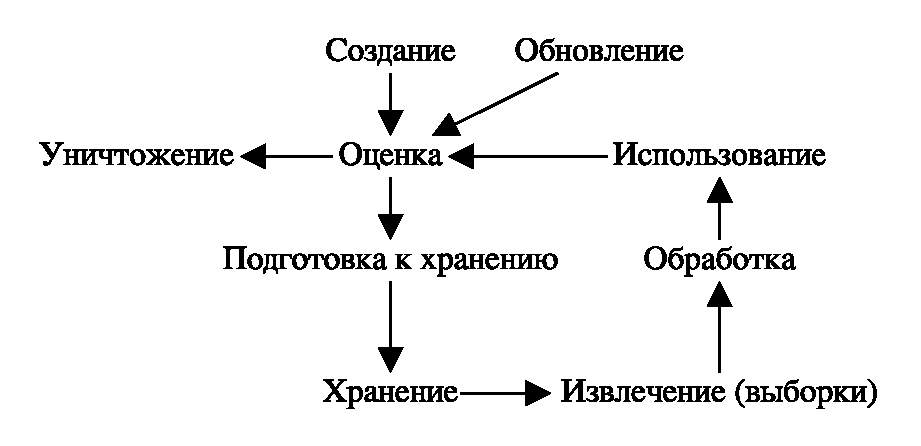
\includegraphics[scale=1]{img/information.pdf}
\end{figure}

\textbf{Документ} -- информация, зафиксированная на материальном носителе, она снабжена реквизитами

\textbf{Электронный документ} -- документированная иформация, представленная в электронной форме.

\textbf{Защита информации} -- принятие мер:

\begin{itemize}
    \item правовые (законы)
    \item организационно-структурные (внутренние правила)
    \item технические (что используется)
\end{itemize}

направленные на:

\begin{enumerate}
    \item предотвращение неправомерных действий

        \begin{itemize}
            \item доступ
            \item копирование
            \item модификация
            \item блокирование
            \item предоставление
            \item распространение
            \item уничтожение
        \end{itemize}

    \item соблюдение конфиденциальности (информация ограниченного доступа)
    \item реализация права доступа к информации
\end{enumerate}

\subsection{Стандарт банка России -- СТО БР ИББС}

\textbf{Активы} -- все, что имеет ценность для субъекта и находится в его распоряжении.

\textbf{Информационная сфера:}

\begin{itemize}
    \item информация
    \item информационная структура
    \item субъекты
    \item процедуры
\end{itemize}

\textbf{Система регулирования} -- контролирующая, чтобы все было безопасно.

\textbf{Угроза} -- опасность, предполагающая возможность потерь или ущерба.

\textbf{Безопасность} -- состояние защищенности в условиях угроз.

\textbf{Информационная безопасность} -- безопасность в условиях угроз в информационной сфере.

Обеспечивает

\begin{itemize}
    \item доступность
    \item целостность
    \item конфиденциальность
    \item ответственность
    \item подотчетность
    \item аутентичность
    \item достоверность
\end{itemize}

\textbf{Индентификация} -- присвоение уникального имени.

\textbf{Аутентификация} -- установление подлинности идентификатора.

\textbf{Авторизация} -- предоставление прав доступа.

\subsection{Активы}

\textbf{Ценность актива} -- меры ущерба, наносимые нарушением безопасности этого актива.

\textbf{Важность актива} бывает:

\begin{itemize}
    \item жизненно важная -- та, без которой система не может функционировать;
    \item важная -- ущерб велик, но система может функционировать без нее;
    \item полезная (рабочая) -- рабочая информация для функционирования, баботать плохо, но можно;
    \item несущественная -- вспомогательные файлы, архивы.
\end{itemize}

\textbf{Что учитывать}

\begin{enumerate}
    \item Простота -- чем проще, тем меньше непротестированных моментов;
    \item Полнота -- закрыть все возможные подходы для нарушения безопасности;
    \item Ответственность -- авторизация, аутентификация, идентификация, если что сделал не так, то имеет ответственность за произошедшее;
    \item Обоснованность доступа -- необходимое и достаточное;
    \item Разграничение потоков информации -- разделять разные уровни секретности (важности) информации;
    \item Чистота повторного использования;
    \item Целостность средств защиты -- сертификаты удостоверяются, что ничего не поменялось.
\end{enumerate}

\subsection{Методы защиты информации}

\begin{enumerate}
    \item \textbf{Системы аутентификации}

        \begin{itemize}
            \item пароль;
            \item ключ доступа;
            \item сертификат;
            \item биометрия;
            \item одноразовые коды;
            \item третья доверенная сторона.
        \end{itemize}

    \item \textbf{Средства авторизации}

        \begin{itemize}
            \item модели доступа;
            \item журналирование.
        \end{itemize}

    \item \textbf{Криптографические средства}

        \begin{itemize}
            \item алгоритм шифроваия;
            \item электронная подпись.
        \end{itemize}

    \item \textbf{Системы анализа и моделирования инфо потоков}

        \begin{itemize}
            \item средста мониторинга;
            \item моделирование с имитацией;
            \item межсетевое экранирование.
        \end{itemize}

    \item \textbf{Антивирусы + регулярное обновления}

    \item \textbf{Регулярное резервное копирование}

    \item \textbf{Резервирование HW}

        \begin{itemize}
            \item железо;
            \item питание.
        \end{itemize}

    \item \textbf{Режимные меры, физическая защита}
\end{enumerate}
